In the last years the interest among data-intensive technologies and applications in order to extract useful information from data has increased in our day to day. These data-intensive applications and their execution environments allow users not only to handle Big Data but also to do it efficiently. This is why Big Data has become in a common technology in our lives.

Furthermore, the appearance of Big Data has generated some needs in our society. One of these needs are privacy policies. DIAs require some tools which are able to preserve the privacy of users which are generating such data. These tools can vary from international laws that legislate in this regard to technical approaches that allow to encrypt the flowing data.

Due to the development of these technologies all together and the wide range of applications where Big Data is still getting involved, writing DIA codes form scratch became in an inefficient task. At this point was where modeling techniques for software development became important for DIA development.

% Ask about this section here or in chapter 2 with references

\section{StreamGen}
StreamGen is a model-driven approach to support the design of DIAs and the automated code generation for two target platforms, Flink and Spark. This approach is developed focusing on two requirements:

\begin{itemize}
\item To provide a platform-independent and graphical modeling language for streaming applications.
\item To enable the fast prototyping of distributed streaming applications over different platforms.
\end{itemize}

The first requirement is needed in order to develop any kind of DIA for different target platforms and, independently for which platform it is targeted, provide a complete language for all of them. This is possible due to the DIA dataflow model characteristic that supports the development of them by means of sources, transformations and sinks. The second requirement is satisfied by using UML class diagrams for such purpose. This kind of diagrams allow to represent sources, transformations and sinks but also the data flows really fast, just introducing the predefined stereotypes.

\subsection{DIA Generation Process}

The different steps that have to be followed in order to generate a DIA with StreamGen are the following:

\begin{itemize}
\item UML model creation.
\item Application code generation.
\item Application execution.
\end{itemize}

\subsubsection*{UML model creation}

First of all, the user must create a UML model by exploiting a predefined language in a UML profile diagram. This language consists of four metaclasses:

\begin{itemize}
\item Class
\item InformationFlow
\item Model
\item Package
\end{itemize}

The class metaclass represents the streaming operators stereotypes which are data sources, data sinks and data stream transformation. Moreover, this three stereotypes can be represented by means of several generalization. In the table \ref{StreamGen Classes} can be shown such stereotypes.

\begin{table}[h!]
\centering
	\begin{tabular}{||c|c|c||} 
	\hline\hline
	Sources & Transformations & Sinks \\ 
	\hline\hline
	Text File & Reduce & Text File \\ 
	\hline
	Socket & Map & CSV File \\ 
	\hline
	Collection & Window & Socket \\ 
	\hline
	Kafka & Flatmap & Cassandra \\ 
	\hline
	 - & NFlatmap & Kafka \\
	\hline
	 - & NMap & - \\
	\hline
	 - & Count & - \\
	\hline
	 - & Fold & - \\
	\hline
	 - & Sum & - \\
	\hline
	 - & Filter & - \\
	\hline
	 - & Join & - \\
	\hline
	 - & CoGroup & - \\
	\hline\hline
	\end{tabular}
\caption{StreamGen Classes}
\label{StreamGen Classes}
\end{table}

The InformationFlow metaclass represents the data streams. There are three main data streams stereotypes: non-parallel stream, windowed stream and partitioned stream. Moreover, the partitioned stream stereotype can be generalized to broadcasted stream, keyed stream, randomly partitioned stream and round robin stream.

The model metaclass is extended by a distributed streaming application stereotype which is generalized to Flink application, Spark application and Apex application.

The last metaclass, the package, is extended by the stream data types stereotype which will contain all the data types conveyed by the different information flows.

\subsubsection*{Application code generation}

Once the user has defined the UML model, the java application configuration must be run in order to generate the application codes. This is possible because of the development of an Acceleo code. This Acceleo program is able to take as inputs the generated UML model and, depending on the different stereotypes contained in such model, generate a DIA code for Flink or Spark.

\subsubsection*{Application execution}

Currently, StreamGen allows code generation for Spark and Flink. As can be seen in its model stereotypes, also there is an intention to develop Apex codes in the future.

\subsection{DIA Examples}

\subsubsection{Great Seller DIA}
Along this document a DIA for an e-commerce company called Great Seller is implemented. This DIA is able to compute real time statistics about the transactions generated by the consumers. Such statistics can be observed by some other companies that pay in order to have access to the information making that Great Seller acts as a data broker. In order to simplify the implementation, Great Seller is going to sell three different types of statistics:

\begin{itemize}

\item Statistic 1: the total amount of money that each consumer of Great Seller spend in the last 10 minutes.
\item Statistic 2: the number of transactions issued by each user in the last 10 minutes.
\item Statistic 3: the number of users who spent more than \euro{1000} in the last hour.

\end{itemize}

As any DIA, Great Seller generates such statistics by some transformations which are fed from a source and the generated information is stored into a sink which is accessible by the observer companies. Moreover, as Great Seller is producing three different types of statistics, its DIA requires three different sinks where the information should be stored. Due to the fact that Great Seller DIA is computing real time statistics about the transactions that are generated by the consumers of the company, only one source is required for the DIA model. Finally, one transformation is necessary for the computation of each statistic. In summary, Great Seller DIA requires one source, three transformations and three sinks for the design of its model.

\subsubsection*{Great Seller Source}
In the implementation described along this document, Great Seller DIA is fed from a socket that reads from a text file where all the transactions generated by the consumers of Great Seller are stored. All the transactions are going to have the same predefined tuple structure 'transactionId,dataSubject,spentAmount,purchasedProduct'. This predefined structure is represented in the Great Seller DIA model by means of a Data Type called InputTransaction.

Regarding to the fields of such tuple, the transactionId field is an integer which varies from 1 to the number of generated transactions, such number can be 10, 100 or 1000. The dataSubject is the user who generates such tuple and it is one of the following: Bob, Carlos, Elisabetta or Michele. The spentAmount is the price paid for the product bought with the transaction and it is an integer with a low boundary of \euro{1} and an upper boundary of \euro{200}. Finally, the purchasedProduct is the product bought with such transaction.

It is important to remark that socket source introduces in the DIA a data stream of string and the InputTransaction Data Type must be generated by means of a transformation which parses the string into the Data Type. This transformation is called TupleParser as it splits the incoming tuples, strings, into the InputTransaction Data Type.

The Great Seller stock is composed by means of 25 products. In order to simplify the implementation, each product is named by the word 'product' immediately followed by a number between 1 and 25 in order to specify the product referred in the stock. In the table \ref{Great Seller Stock} can be seen such stock.

\begin{table}[h!]
\centering
	\begin{tabular}{||c|c||} 
	\hline\hline
	Product & Price (\euro{}) \\ [1ex] 
	\hline\hline
	product1 & 196 \\ 
	\hline
	product2 & 36 \\ 
	\hline
	product3 & 179 \\ 
	\hline
	product4 & 17 \\ 
	\hline
	product5 & 120 \\ 
	\hline
	product6 & 187 \\ 
	\hline
	product7 & 139 \\ 
	\hline
	product8 & 52 \\ 
	\hline
	product9 & 160 \\ 
	\hline
	product10 & 110 \\ 
	\hline
	product11 & 113 \\ 
	\hline
	product12 & 67 \\ 
	\hline
	product13 & 100 \\ 
	\hline
	product14 & 125 \\ 
	\hline
	product15 & 192 \\ 
	\hline
	product16 & 115 \\ 
	\hline
	product17 & 113 \\ 
	\hline
	product18 & 98 \\ 
	\hline
	product19 & 113 \\ 
	\hline
	product20 & 185 \\ 
	\hline
	product21 & 143 \\ 
	\hline
	product22 & 18 \\ 
	\hline
	product23 & 194 \\ 
	\hline
	product24 & 41 \\ 
	\hline
	product25 & 26 \\ 
	\hline\hline
	\end{tabular}
\caption{Great Seller Stock}
\label{Great Seller Stock}
\end{table}

\subsubsection*{Great Seller Transformations}
In order to compute each of the three statistics that Great Seller sells as data broker, the Great Seller DIA needs three transformations. Each of this transformations is the operator of each statistic. Thus, the operator one (OP1) computes the total amount of money spent by each user in the last 10 minutes. The second operator (OP2) computes the number of transactions issued by each user in the last 10 minutes. Finally, the operator three (OP3) computes the number of users who spent more than \euro{1000} in the last hour.

These transformations input a data stream with a set of tuples that all of them have identical structure. Thus, the first stream (S1) is composed of tuples of the kind InputTransaction. This stream is duplicated and it is sent to the operators OP1 and OP2. Moreover, as each operator works taking into account the data subject of each tuple, the stream S1 must be keyed by the data subject field of this first stream. Finally, as the operators have to compute the statistics taking into account only the tuples generated in the last 10 minutes, the stream S1 is windowed by a time window of 10 minutes.

The new data generated in the OP1 are represented in a new data type called SpentAmount and that is composed by two fields following the structure: 'dataSubject, totalAmount'. The SpentAmount tuples are collected in the stream S2 and they are keyed by the data subject field of such stream.

Finally, the data generated in the OP2, is collected in a new data type called IssuedTransaction whose structure is 'dataSubject, nTransactions'. This new stream (stream S3) is sent to the OP3. Moreover, this third stream is keyed by the data subject field of the stream and it is also windowed with a time window of one hour. The OP3 generates a randomly partitioned stream with an uniform distribution called stream S4 whose structure is: 'nTopUsers'.

\subsubsection*{Great Seller Sinks}
Each of the tuples flowing through the DIA must be stored in a file, in order to be able to access to the tuples that will be sent to the observer companies. This is why, after each generated stream, a file text sink is implemented with different paths in order to store each of the flows obtaining all the results in three different files. The file with the results of the stream S2, the stream S3 and the stream S4.
This implementation is given due to the fact that each of the tuples generated by the operators are observable for the observer companies who buy them.

In the figure \ref{fig:Great Seller Dataflow model} the dataflow model of the Great Seller DIA without privacy policies can be seen. This dataflow model can be found in \cite{privacypoliciesarticle}. On the other hand, in the figure \ref{fig:Great Seller StreamGen DIA} the model developed with StreamGen taking into account the figure \ref{fig:Great Seller Dataflow model} can be seen for such DIA.

\begin{figure}
\centering
{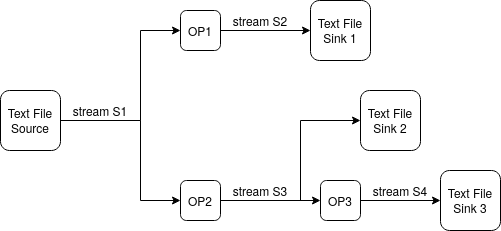
\includegraphics[scale=0.5]{./chapter3/greatSellerApp.png}}
\caption{Great Seller Dataflow model}
\label{fig:Great Seller Dataflow model}
\end{figure}

\begin{figure}
\centering
{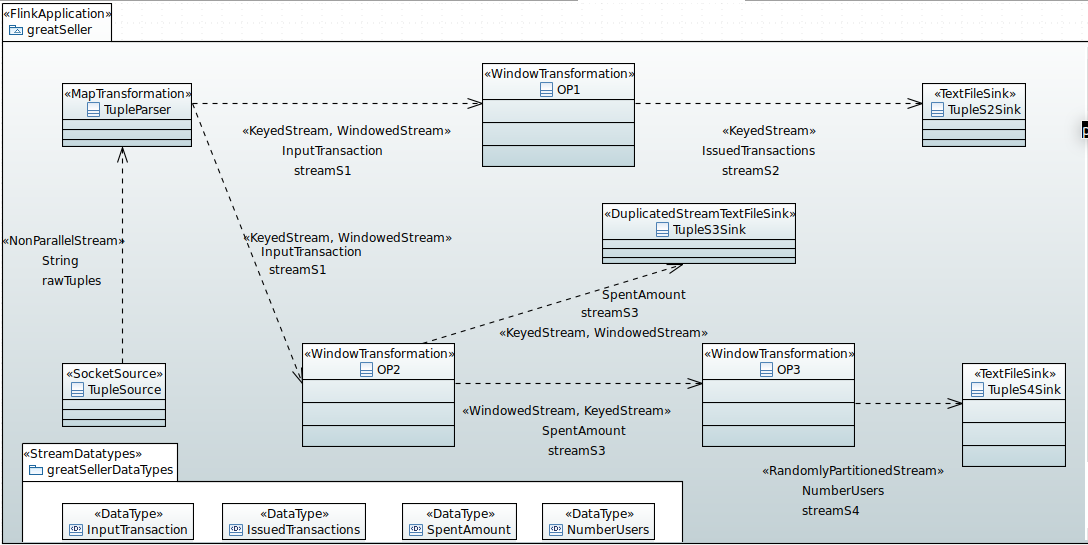
\includegraphics[scale=0.3]{./chapter3/greatSellerStreamGen.png}}
\caption{Great Seller StreamGen DIA}
\label{fig:Great Seller StreamGen DIA}
\end{figure}

\subsubsection*{Great Seller DIA Limitations}

After developing this DIA, some limitations are identified relative to the current development of StreamGen. The first limitation is the number of server that can be connected directly to a Map Transformation. In this example, it is supposed that the users send the transactions by means of a server to the target DIA. This server is the same for all the users who are using Great Seller DIA. At this point, a casuistry is proposed. This is the case of a DIA involved in an industry 4.0 application where the owner of the factory cannot afford to invest in a server for the DIA and all the machines generating datasets must be connected directly to the DIA by means of the factory net.

The second limitation that is extracted is that StreamGen does not allow to generate float or double data types. In this example, Great Seller is working with a stock where all the products have integer prices but should be necessary a DIA which allows, among the language, to declare float or double values.

The last extracted limitation is that StreamGen is not able to handle the privacy of the users who are using the DIA. In this case, neither the language for such purpose nor the translation by means of Acceleo are available. After the development of both things, this model should be reused in order to make the application privacy aware.

\subsubsection{Cool Analyst DIA}

In addition to Great Seller, another DIA is developed with StreamGen. This is the case of Cool Analyst, a DIA which is able to compute some statistics from the temperatures measured in two different refrigeration chambers of a panettone factory called Panettone 4.0. These measurements are going to be stored in a CSV file in order to be accessible by the manager of the industrial plant to see if any problem has been produced in the yeast fermentation. This application is going to compute four statistics in two different operators:

\begin{itemize}
\item Operator 1: the maximum, the minimum and the average temperature of each chamber during the last 5 minutes.
\item Operator 2: the prediction of the temperature for the next 10 minutes.
\item Operator 3: the filtered data between a range which have no null value and no null id.
\end{itemize}

Cool Analyst DIA is going to require two socket sources, one for each of the industrial chambers, two transformations in order to compute each of the operators specified before and two sinks where the CSV files with each of the results of the operators can be stored. For the development of the prediction operator, as its development is out of this document, it is taken from an already working transformation for such purpose.

\subsubsection*{Cool Analyst Sources}

Panettone 4.0 is using temperature digital sensors in each of its two chambers where yeasts are fermented. These sensors are connected to the net of the factory and are sending the measured values directly to the Cool Analyst DIA with a 1 second sample frequency.

This two chambers need to control the temperature of the room in order to allow the correct fermentation of the yeasts. The role of the first chamber is to make the primary fermentation in the production process of the Panettone 4.0 factory. This fermentation is also known as bulk fermentation. On the other hand, the role of the second camera is to make the secondary fermentation which is also known as proofing. More information can be read about the fermentation of the years and how to control the temperature during its production in \cite{yeastfermentation}. The conclusions that are extracted from \cite{yeastfermentation}, and that are useful for our purpose, are that the bulk fermentation must have the temperatures of the room in the range [20, 24] Celsius whilst the secondary fermentation must have an environment with temperatures in the range [22, 29] Celsius. This is why Cool Analyst requires two socket sources connected to the port and to the host of each of the chambers.

Also it is important to remark how the temperatures of the chambers are simulated. For such purpose a python code has been developed. This model takes as target temperature, the average temperature of each of the ranges. This temperature is supposed to be maintained during thirty seconds. Then, randomly, the program generates a sine function with a frequency of 1/16 Hz for the lower range and with a frequency of 1/28 Hz for the upper range. The lower range is considerate from the lower boundary of each of the ranges of temperature that the chambers can admit until the average temperature and the upper range from the average temperature until the upper boundary of the ranges. In the figures \ref{fig:Temperature Chamber 1 Model} and \ref{fig:Temperature Chamber 2 Model} can be seen both models.

\begin{figure}
\centering
{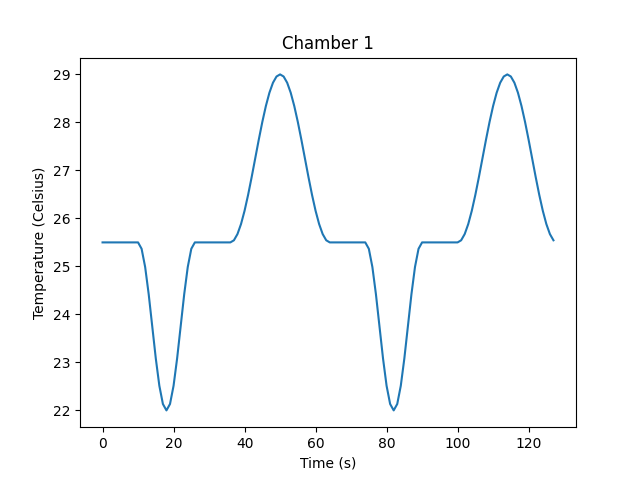
\includegraphics[scale=0.3]{./chapter3/room1TempModel.png}}
\caption{Temperature Chamber 1 Model}
\label{fig:Temperature Chamber 1 Model}
\end{figure}

\begin{figure}
\centering
{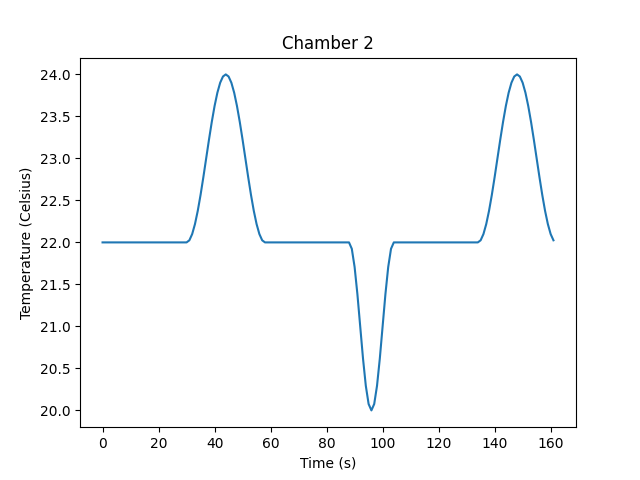
\includegraphics[scale=0.3]{./chapter3/room2TempModel.png}}
\caption{Temperature Chamber 2 Model}
\label{fig:Temperature Chamber 2 Model}
\end{figure}

Finally, these two models have been generated and saved in a TXT file which is going to be read from the Python servers that have been developed in order to simulate the chambers. These servers are going to read one value each second. This will generate that the socket sending the values from the chamber 1 stops earlier than the other socket. This model design will allow to proof the right behavior of the whole application. Allowing to see what would happen if, suddenly, the sensors are disconnected.

\subsubsection*{Cool Analyst Transformations}

The values read from the TXT file are sent in a string which has to be parsed in order to generate the Data Types that are used in the DIA. The strings contain the roomId followed by the temperature and both values are separated by means of a comma. This is why, first of all a NMap Transformation has been developed, this will be explained in the following chapter. This NMap transformation inputs the two streams with the strings sent by the room servers and the string is parsed into a roomTemp data type which is composed of two properties: roomId (string) and roomTemp(double). In order to introduce double values from the Papyrus model by means of StreamGen, in chapter 4 is explained how StreamGen was modified.

Once the roomTemp data type is generated, a stream is sent to a window transformation called RoomStatistics. In this transformation all the computations explain in the operator 1 are calculated (maximum temperature, minimum temperature and average temperature). This transformation generates a new data type called roomStatistics which is composed of four properties: roomId (string), maxTemp (double), minTemp (double) and avgTemp (double).

Then, the stream with the roomStatistics data types is sent to the TemperaturePredictor transformation. This window transformation computes the operations described in the operator 2 and generates the tempPred data type. This data type is composed of two properties: roomId (string) and predTemp (double).

The last operator takes the stream with the roomTemp data type and, by means of a filter transformation called CleanRawData, checks that there is no temperature with a value below -9999 neither 9999. Moreover, this transformation checks that the temperature has a value and that value is referenced to a room identifier.

\subsubsection*{Cool Analyst Sinks}

Finally, the data types generates in the RoomStatistics, in the TemperaturePredictor and in the CleanRawData transformations are stored each one in its sink. Cool Analyst uses CSV sinks as this kind of files are commonly used by engineers who work in the factories. In order to do this, the output stream from the RoomStatistics transformation is sent to StatisticsSink where is specified the path of the generated file, the output stream from the TemperaturePredictor transformation is sent to PredictorSink where the path of the second output file is specified and the same proceadure is done with the third operator CleanRawData and its sink CleanDataSink.

In the figures \ref{fig:Cool Analyst Dataflow model} and \ref{fig:Cool Analyst StreamGen DIA} can be seen the Cool Analyst Dataflow Model and the Cool Analyst StreamGen DIA explained above.

\begin{figure}
\centering
{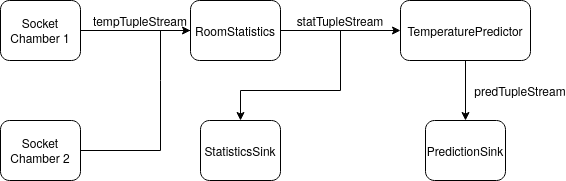
\includegraphics[scale=0.5]{./chapter3/coolAnalystApp.png}}
\caption{Cool Analyst Dataflow model}
\label{fig:Cool Analyst Dataflow model}
\end{figure}

\begin{figure}
\centering
{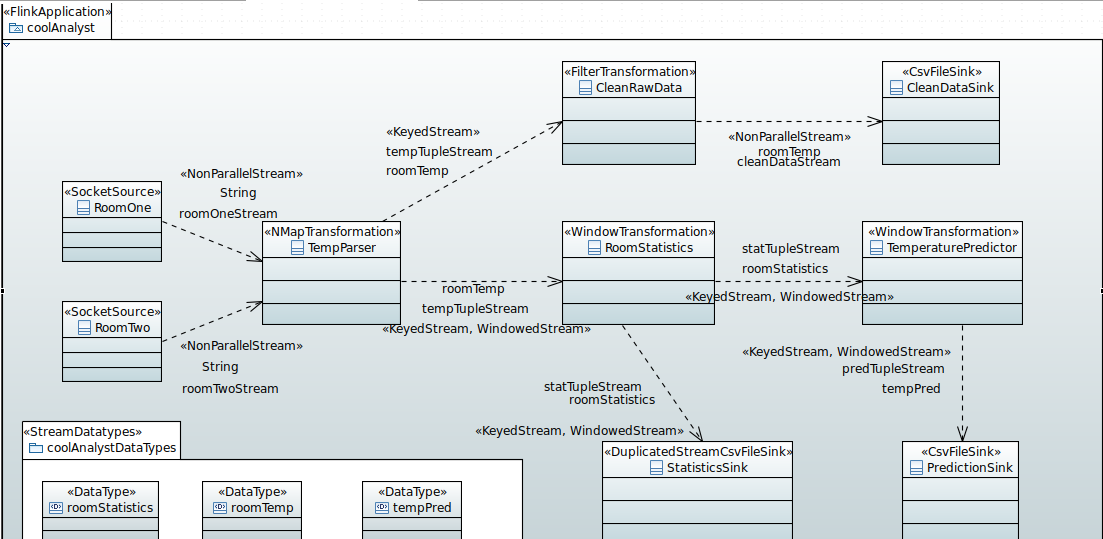
\includegraphics[scale=0.3]{./chapter3/coolAnalystStreamGen.png}}
\caption{Cool Analyst StreamGen DIA}
\label{fig:Cool Analyst StreamGen DIA}
\end{figure}

\subsubsection*{Great Seller DIA Limitations}

At this example two of the limitations identified with the previous DIA are already solved. This is the case of the NMap Transformation and the possibility to generate double values by means of Papyrus. This will be seen in the following chapter.

However, StreamGen is still not able to handle the privacy of the users who are using the DIA. This is why this DIA will be reused, as Great Seller, after the development of the language and the Acceleo code to test StreamGen for privacy purposes.
